\subsection{Verfahren des maschinellen Lernens}
\label{subsubsec_Verfahren}
Es existieren viele konkrete Algorithmen des MLs, welche sich in eine oder mehrere der vorher genannten Typen einordnen lassen. Folgend werden die theoretischen Grundlagen der jeweiligen Algorithmen erläutert. Die in der Literatur und Praxis häufig genannten ML-Verfahren sind: Entscheidungsbäume, logistische Regression, Bayessche Modelle, Support Vector Machines, k-means Clustering, k-nearest Neighbours sowie neuronale Netze \cite{alzubi2018machine, MicrosoftML, dobel2018maschinelles, sarker2021machine}. \todo[noline]{Diese Auswahl am Ende noch einmal überdenken/anpassen} Um den Umfang nicht zu sprengen, wird sich auf diese häufig genannten konzentriert.
%Fraunhofer Quelle hat sogar eine Befragung gemacht

\subsubsection{Entscheidungsbäume}
\label{chap_dectree}
\begin{wrapfigure}{r}{0.5\textwidth}
    \centering
    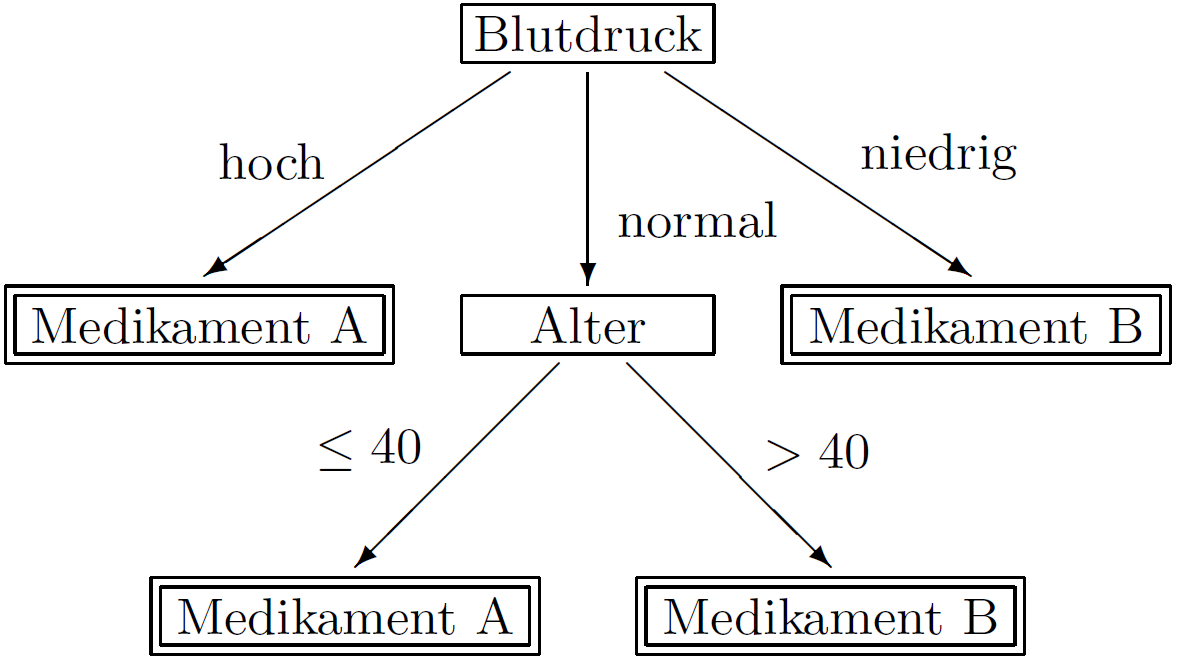
\includegraphics[scale=0.33]{pic/MA-Bilder/Entscheidungsbaum.PNG}
    \caption{Beispiel für einen Entscheidungsbaum \cite{borgelt1998attributauswahlmasse}}
    \label{Fig:dectree}
\end{wrapfigure}
Entscheidungsbäume können zur Klassifikation oder Regression eingesetzt werden \cite{Wuttke.2022}. Entscheidungsbäume, welche zur Klassifikation eingesetzt werden, teilen eine Menge immer wieder in unterschiedliche Teilmengen auf. Die letzte Unterteilung entspricht der Klasse zu der eine Entität gehört \cite{Breiman.2017}. Bei dieser schrittweisen Aufteilung spricht man auch von rekursiver Partitionierung \cite{Ng.2018}. Soll ein Entscheidungsbaum konstruiert werden, kann wie folgt vorgegangen werden: man starte zunächst mit der Wurzel, die ein erstes Entscheidungskriterium beinhaltet. Von dieser Wurzel aus können mehrere Kanten ausgehen, welche zu anderen Knoten führen. An diesen Knoten können sich wiederum Entscheidungskriterien mit neuen Kanten befinden. Knoten ohne Nachfolger bilden die Blätter und somit auch die Kategorien des zugrundeliegenden Klassifikationsproblems \cite{Wuttke.2022}. Ein Beispiel für einen Entscheidungsbaum ist in Abbildung \ref{Fig:dectree} zu sehen.

Entscheidungsbäume haben jedoch einige Nachteile, so können geringe Änderungen im Trainingsdatensatz große Auswirkungen im Design des Baumes nach sich ziehen. Überdies können unglücklich ausgewählte binäre Entscheidungskriterien am Baumknoten ungenaue Endergebnisse hervorrufen. Abhilfe kann eine mögliche Abwandlung von Entscheidungsbäumen schaffen, welche die Komplexität des Algorithmus jedoch erhöht. Dieses Verfahren heißt \enquote{Random Forest}, da dort verschiedene, zufällig erzeugte Entscheidungsbäume zur gleichen Zeit arbeiten. Am Ende werden über die Ergebnisse aller Bäume ein Mittelwert gebildet oder auf andere Weise zu einer endgültigen Antwort zusammengefasst \cite{Ng.2018}.

\subsubsection{k-means Clustering}
\label{subsubsec:k-means-Clustering}
\begin{wrapfigure}{r}{0.5\textwidth}
    \centering
    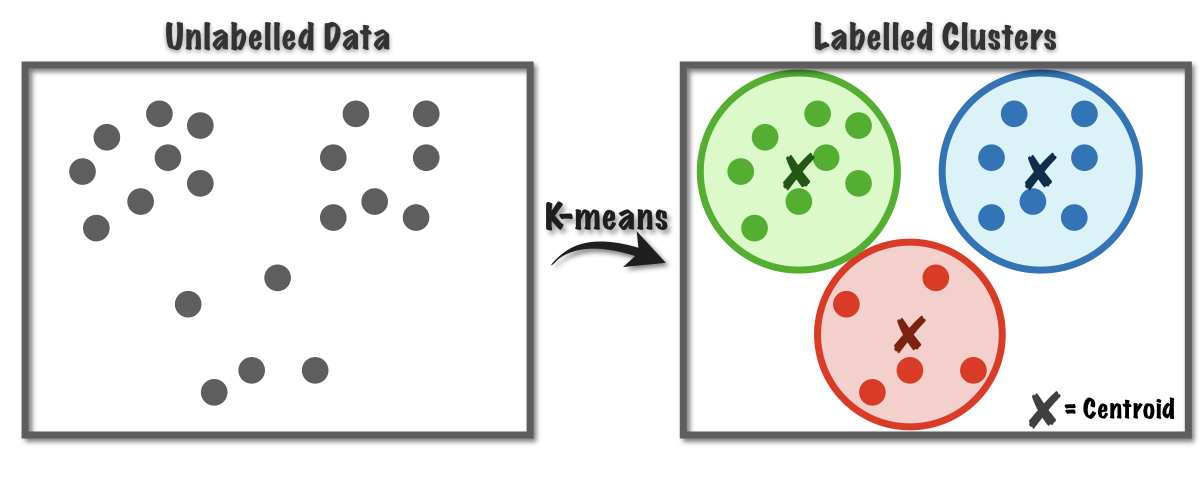
\includegraphics[scale=0.16]{pic/MA-Bilder/k-means-Clustering.png}
    \caption{Input und Output des \emph{k-means Clustering}-Verfahrens, entnommen aus \cite{Fiori-online}}
    \label{Fig:kmeans}
\end{wrapfigure}
Das \emph{k-means Clustering}-Verfahren ist ein Algorithmus des unüberwachten Lernens und kann bspw. dazu eingesetzt werden gezielte Werbestrategien zu entwickeln \cite{Matzka.2021, Ng.2018}. So können Kunden, die bestimmte Merkmale, z.B. Einkommen oder Persönlichkeitszüge wie Offenheit gemeinsam haben, die gleichen Produkte vorgeschlagen werden \cite{Ng.2018}. Das \emph{k-means Clustering}-Verfahren unterstützt dies, indem es Kunden (oder universell formuliert Datenpunkte) einem von $k$ Clustern zuordnet \cite{ayodele}. $k$ muss bei diesem Verfahren vorgegeben werden. Im Fokus des Verfahrens steht die Ermittlung der Zentren (engl.: \emph{Centroide}) eines jeden Clusters \cite{Cleve.2020}.
\newline

Die Funktionsweise des Verfahrens lässt sich in etwa wie folgt umreißen: zu Beginn werden (zufällig) die Standorte der $k$ Zentren gewählt \cite{Cleve.2020}. Als nächstes wird für jeden Datenpunkt das ihm am nächsten liegende Zentrum gefunden. Ist dies für jeden Datenpunkt erfolgt, werden neue Zentren ermittelt, indem die Mittelpunkte aller einem Zentrum zugehörigen Datenpunkte berechnet werden. Als nächstes folgt eine erneute Zuordnung aller Datenpunkte zu den neuen Zentren. Diese Zuordnung und Zentrenbildung wird so lange wiederholt bis sich keine neuen Zentren mehr auffinden lassen \cite{Ng.2018}. Abbildung \ref{Fig:kmeans} visualisiert das Endergebnis des \emph{k-means Clustering}-Verfahrens beispielhaft.

 \emph{k-means Clustering} ist aufgrund seiner geringen Komplexität während der Implementierung beliebt. Vereinfacht gesagt, müssten bei einer Realisierung des Algorithmus nur immer wieder neue Abstände berechnet werden und draufhin die Datenpunkten (erneut) den Clusterzentren zugeordnet werden \cite{Cleve.2020}. Neben dieser Einfachheit existieren jedoch auch einige Schwächen, wie z.B. die Form der Cluster. Durch die iterative Anwendung entstehen kreisförmige Cluster. In der Realität ist es jedoch nicht selten, dass die realen Cluster ein anderes, z.B. elliptisches Erscheinungsbild besitzen \cite{Ng.2018}.  Weiter ist der Algorithmus anfällig in Bezug auf Rauschen und Ausreißer \cite{Cleve.2020}. Als Ausreißer bezeichnet man Datenpunkte, welche sich von den anderen stark unterscheiden. Ein Beispiel hierfür könnten Kundendaten sein, welche das Alter der Personen beinhalten. Wären alle Kunden 20-30 Jahre alt, aber gäbe es einen Kunden, welcher 80 Jahre als ist, wäre dies der Ausreißer \cite{Cleve.2020}. Rauschen in Daten kann sich in Form verschiedenster Anomalien bemerkbar machen. Beispielsweise kann es zu Messfehlern bei der Datenbeschaffung gekommen sein, wohingegen auch die Betrachtung zu vieler Attribute beim Lernprozess ein Rauschen verursachen kann \cite{Alpaydin+2019}. Daneben ist es nicht vorgesehen, dass sich Cluster gegenseitig überlappen \cite{Ng.2018}. Weiter sei angemerkt, dass die Ermittlung von $k$, also die Anzahl der Cluster, nicht durch das Verfahren gelöst wird und diese Entscheidung durch den Anwender getroffen werden muss \cite{Cleve.2020}.
 
 \subsubsection{Support Vector Machines}
 \begin{wrapfigure}{r}{0.5\textwidth}
    \centering
    \raisebox{0pt}[\dimexpr\height-0.7\baselineskip\relax]{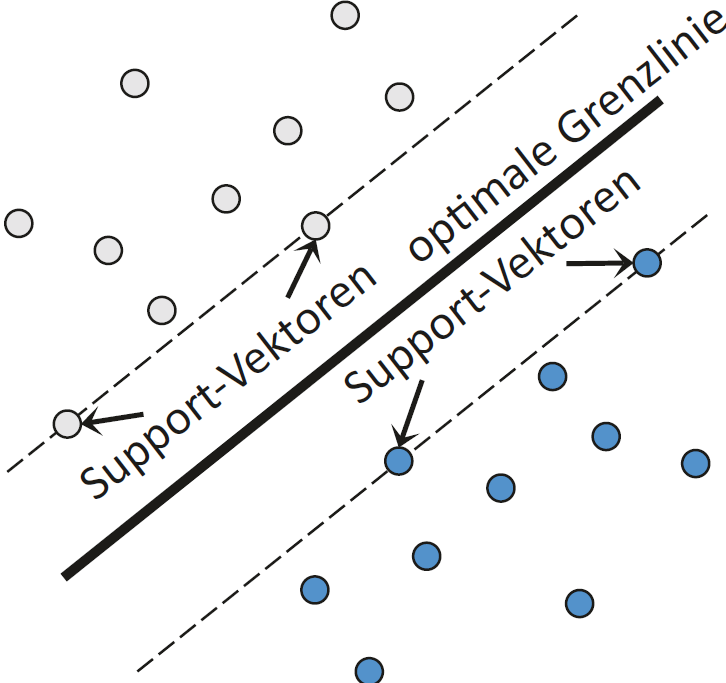
\includegraphics[scale=0.3]{pic/MA-Bilder/support-vector-machines.PNG}}
    \caption{SVM \cite{Ng.2018}}
    \label{Fig:svm}
\end{wrapfigure} 
\emph{Support Vector Machines} (SVM) können zur Klassifikation eingesetzt werden und gehören zu den Algorithmen des überwachten Lernens \cite{Verdhan.2020}. Ziel des Algorithmus ist die Ermittlung einer Grenzlinie (engl.: \emph{Hyperplane}), welche die Datenpunkte zweier oder mehrerer Klassen separiert \cite{Ng.2018, noble2006support}. Im zwei-dimensionalen Raum kann man sich die Separierung der Daten als Gerade vorstellen \cite{Verdhan.2020}. Zur Ermittlung der Grenzlinie ist es erforderlich \enquote{diejenigen Datenpunkte am Rand ihrer jeweiligen Gruppe zu finden, die am nächsten zu den Punkten der jeweils anderen Gruppe gelegen sind} \cite{Ng.2018}. Diese Randpunkte werden als \emph{Support-Vektoren} bezeichnet. Werden die Randpunkte der jeweiligen Klassen verbunden, entstehen zwei Linien. In der Mitte dieser zwei Linien, liegt nun die Hyperplane, was in Abbildung \ref{Fig:svm} visualisiert ist \cite{Ng.2018}. Der SVM-Algorithmus hat folglich zur Aufgabe die Abstände zwischen den \emph{Support-Vektoren} zu maximieren, um die optimale Grenzlinie zu ermitteln, welche die Klassifikation unbekannter Datensätze ermöglicht \cite{Matzka.2021}.

SVM zeichnet ihre Flexibilität in der Separierung aus. Während in Kapitel \ref{chap_dectree} angemerkt wurde, dass das \emph{k-means Clustering}-Verfahren die gefundenen Cluster nur kreisförmig darstellen kann, ermöglicht es die \emph{Kernel}-Taktik hingegen mit SVM auch andere Formen darzustellen. Hierbei kommt es zu einer leichten Abwandlung des Verfahrens, sodass der Algorithmus in höheren Dimensionen angewendet wird und somit z.B. elliptische Abgrenzungen anstatt Geraden ermöglicht werden \cite{Ng.2018}. Weiter können auch Klassifikationen im $n$-dimensionalen Raum mithilfe einer Ebene, welche die Dimension $n-1$ besitzt, realisiert werden \cite{Cleve.2020}. Ein weiterer Vorteil der SVM besteht in der Rigorosität gegenüber Ausreißern durch bestimmte Anpassungen des Verfahrens. So besteht die Möglichkeit Daten, die sowohl nah an der einen als auch an der anderen Gruppe liegen, lediglich mit gewissen Wahrscheinlichkeit einer Gruppe zuzuordnen. Diese Wahrscheinlichkeiten lassen sich durch die Betrachtung des Abstandes zur Grenzlinie berechnen \cite{Ng.2018}.

\subsubsection{Logistische Regression}
\begin{wrapfigure}{r}{0.4\textwidth}
    \centering
    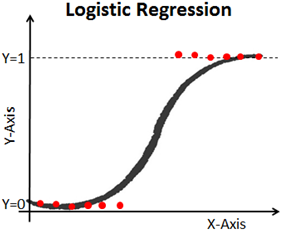
\includegraphics[scale=0.9]{pic/MA-Bilder/logistische-Regression.png}
    \caption{Logistische Regression \cite{Ng.2018}}
    \label{Fig:logistic regression}
\end{wrapfigure}
Die logistische Regression verfolgt das Ziel die Wahrscheinlichkeit des Auftretens einer binären Zielgröße vorherzusagen. Diese Vorhersage kann abhängig von bestimmten Merkmalen getroffen werden. Ein beispielhaftes Szenario, mit dem sich logistische Regression beschäftigen könnte, besteht darin auf Grundlage von Geschlecht und Blutwerten vorherzusagen, wie wahrscheinlich es ist, dass eine Person erkrankt oder nicht erkrankt \cite{Kalisch.2021}. Anders als der Name des Verfahrens logistische \enquote{Regression} vermuten lässt, geht es hier weniger um Regression, sondern eher um Klassifikation \cite{Kersting.2019}. Zur Vorhersage der Wahrscheinlichkeiten wird eine logistische Funktion erstellt. Anders als es in der linearen Regression, in der versucht wird konkrete Werte mithilfe einer Geraden darzustellen, gefordert, ermöglicht es die logistische Funktion Wahrscheinlichkeiten abzubilden \cite{Behnke.2015}. Durch ihr s-förmiges Erscheinungsbild ist diese Funktion in der Lage \enquote{reelwertige Variablen} $[+\infty, -\infty]$ in den Wertebereich von 0 bis 1 zu transformieren \cite{Backhaus.2016}. Die entsprechenden Funktionsparameter der gewünschten logistischen Zielfunktion lassen sich mit der sogenannten \emph{Maximum-Likelihood}-Methode finden \cite{Backhaus.2016}. Diese Methode nähert sich iterativ den Parametern an und sucht diejenige Konstellation der Funktionsparameter, bei der es am wahrscheinlichsten ist, dass die im Trainingsdatensatz vorhandenen Beobachtungen auftreten \cite{Behnke.2015}.

\subsubsection{k-Nächste Nachbarn}
\label{subsubsec_KNN}
\begin{wrapfigure}{R}{0.4\textwidth}
    \centering
    \raisebox{0pt}[\dimexpr\height-1.5\baselineskip\relax]{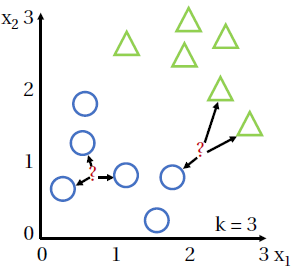
\includegraphics[scale=0.7]{pic/MA-Bilder/k-naechste-Nachbarn.PNG}}
    \caption{Beispiel für kNN mit k=3 \cite{Matzka.2021}}
    \label{Fig:knearest}
\end{wrapfigure}
Das \emph{k-nächste Nachbarn}-Verfahren (kNN) als ML-Algorithmus des überwachten Lernens kann zur Lösung von Klassifikationsproblemen herangezogen werden. Bei der Zuordnung unbekannter Entitäten zu einer Klasse macht kNN sich bestehende Ähnlichkeiten zu bereits zugeordneten Entitäten zu Nutze \cite{Matzka.2021}. Ein herausstellendes Merkmal dieses Verfahrens besteht darin, etwas von dem in Kapitel \ref{subsec_AblaufML} beschrieben Datenfluss abgewichen wird. Bei diesem Algorithmus wird in der Trainingsphase kein Modell erstellt, welches später Zuordnungen vornehmen kann, sondern die Berechnungen und die Klassifikation einzelner Datensätze finden zum selben Zeitpunkt statt \cite{Verdhan.2020, Matzka.2021}. Bei der Bestimmung der Klassenzugehörigkeit, prüft das kNN-Verfahren, wie weit dieser von anderen bereits klassifizierten Datensätzen entfernt ist \cite{Verdhan.2020}. Der Parameter $k$ in kNN steht für die Anzahl der Nachbarn, welche betrachtet werden sollen. Wird $k=1$ gewählt, bestimmt lediglich der nächste Nachbar das Klassenlabel. Wird sich bei der Implementierung für $k=n$ entschieden, fließen die n nächsten Nachbarn in die Entscheidungsbildung mit ein \cite{Matzka.2021}. In Abbildung \ref{Fig:knearest} ist die Funktionsweise des Verfahrens für $k=3$ beispielhaft abgebildet. An dieser Stelle sei angemerkt, dass die Bestimmung von $k$ wichtig für eine angemessene Funktionsweise des Verfahrens ist. Wird k ein kleiner Wert zugewiesen, wird sich bei der Klassenbildung nur auf wenige Daten gestützt, was besonders häufig zu Fehlklassifikation führen kann. Haben jedoch zu viele nächste Nachbarn an der Entscheidungsfindung ihren Anteil, werden Muster unter Umständen nicht präzise genug abgebildet. Neben der Festsetzung des Parameters k besteht eine wichtige Entscheidung darin, wie bei $k\geq 2$ entschieden wird, sollten Nachbarn unterschiedliche Klassenlabels besitzen. Eine Möglichkeit besteht darin, die Klassen aller k-nächsten Nachbarn in die Entscheidung miteinzubeziehen, indem der Mittelwert aller betrachteten Klassen gebildet wird. Alternativ dazu kann es jedoch auch als sinnvoll erachtet werden, solchen Nachbarn, für die eine geringere Distanz gemessen wurde, eine größere Wichtigkeit zuzusprechen \cite{Ng.2018}.

Neben seiner leichten Implementierung hat das kNN-Verfahren den Vorteil, dass es zur Erkennung von Ausreißern genutzt werden kann \cite{Ng.2018, Verdhan.2020}. Eine Schwierigkeit, welche dieses Verfahren jedoch mit sich bringt, ist die Abhängigkeit vom Wert $k$. Dieser trägt viel zu der Präzision der Vorhersagen bei, wohingegen er gleichzeitig nicht leicht zu bestimmen ist. Ferner können sich überlappende Klassen mithilfe von kNN nicht berücksichtigt werden. Dazu ist der Algorithmus langsam und rechenintensiv, da für jeden Punkt zunächst alle Abstände berechnet werden müssen und zusätzlich ein (gewichtetes) Mittel bestimmt werden muss \cite{Verdhan.2020}.

\subsubsection{Bayessche Netze}
Bayessche Netze können Prognosen für Größen, das Eintreffen bestimmter Ereignisse oder die Zugehörigkeit zu einer Klasse abgeben \cite{Dorn.2018, dehen2012bayes}. Ein bayessches Netz betrachtet Variablen und deren Abhängigkeiten zueinander, um Wahrscheinlichkeitsaussagen zu treffen. Bayessche Netze basieren auf dem Satz von Bayes \cite{dobel2018maschinelles}. Dieser Satz trifft Aussagen darüber, wie wahrscheinlich es ist, dass ein bestimmtes Ereignis eintritt, unter der Bedingung, dass ein anderes Ereignis eingetreten ist \cite{Dorn.2018}. Bayessche Netze sind gerichtete Graphen, welche diesen Satz anwenden \cite{Dorn.2018, dobel2018maschinelles}. In solchen Graphen stellen die Knoten Ereignisse oder Größen dar, während die Kanten die Abhängigkeiten der verschiedenen Knoten abbilden. Jeder Knoten besitzt mindestens zwei mögliche Zustände, wie z.B. wahr oder falsch. Darüber hinaus werden den Knoten Wahrscheinlichkeitswerte in tabellarischer Form zugewiesen. In diesen Netzen können bestimmte Arten von Beziehungen existieren. So kann ein Ereignis ein anderes bedingen. Auch möglich ist, dass mehrere vorgeschaltete Ereignisse in Kombination Auswirkungen auf ein weiteres haben \cite{dehen2012bayes}. In der Abbildung \ref{Fig:bnetz} ist ein simples bayessches Netz dargestellt. Bei bewölkten Wetter ist es sehr wahrscheinlich, dass es regnet, während es weniger wahrscheinlich ist, dass ein Rasensprenkler gestartet wird. Regen und ein Rasensprenkler in Kombination bedingen mit hoher Wahrscheinlichkeit, dass der Rasen nass wird \cite{dobel2018maschinelles}. Auf Grundlage von (kausalen) Beziehungen kann also die Wahrscheinlichkeit für das Eintreten eins bestimmten Ereignisses (Nasses Gras) berechnet werden, wenngleich die Wahrscheinlichkeit für genau dieses Ereignis - \enquote{Nasses Gras} - im Vorhinein nicht bekannt war \cite{dobel2018maschinelles, dehen2012bayes}. Die entsprechenden Werte lassen sich mithilfe des Satz von Bayes berechnen \cite{dehen2012bayes}.
\begin{figure}
    \centering
    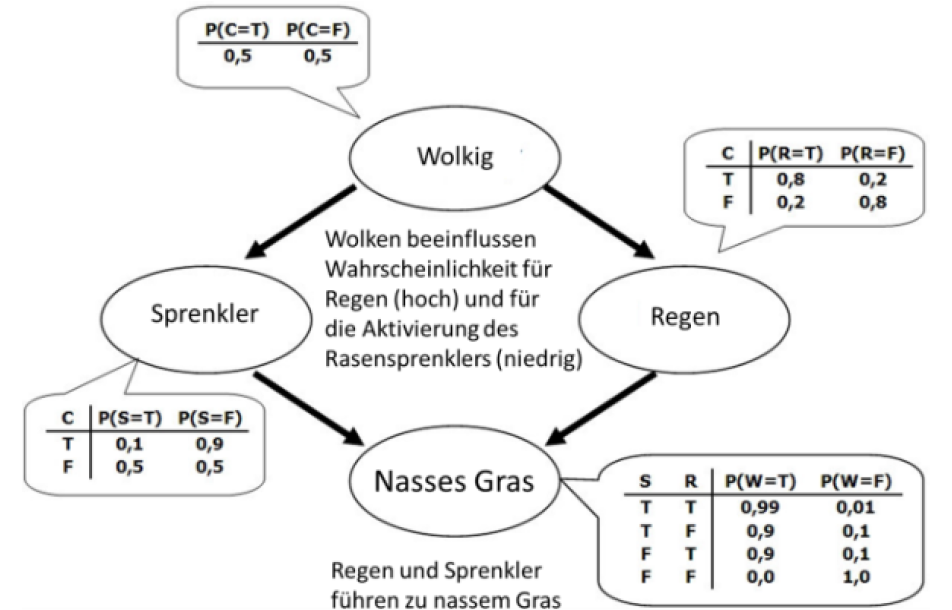
\includegraphics[scale=0.5]{pic/MA-Bilder/bayesNetz.PNG}
    \caption{Beispiel für Bayessche Netze, entnommen aus \cite{dobel2018maschinelles}}
    \label{Fig:bnetz}
\end{figure}%

\begin{wrapfigure}{r}{0.48\textwidth}
    \centering
    \raisebox{0pt}[\dimexpr\height-1.9\baselineskip\relax]{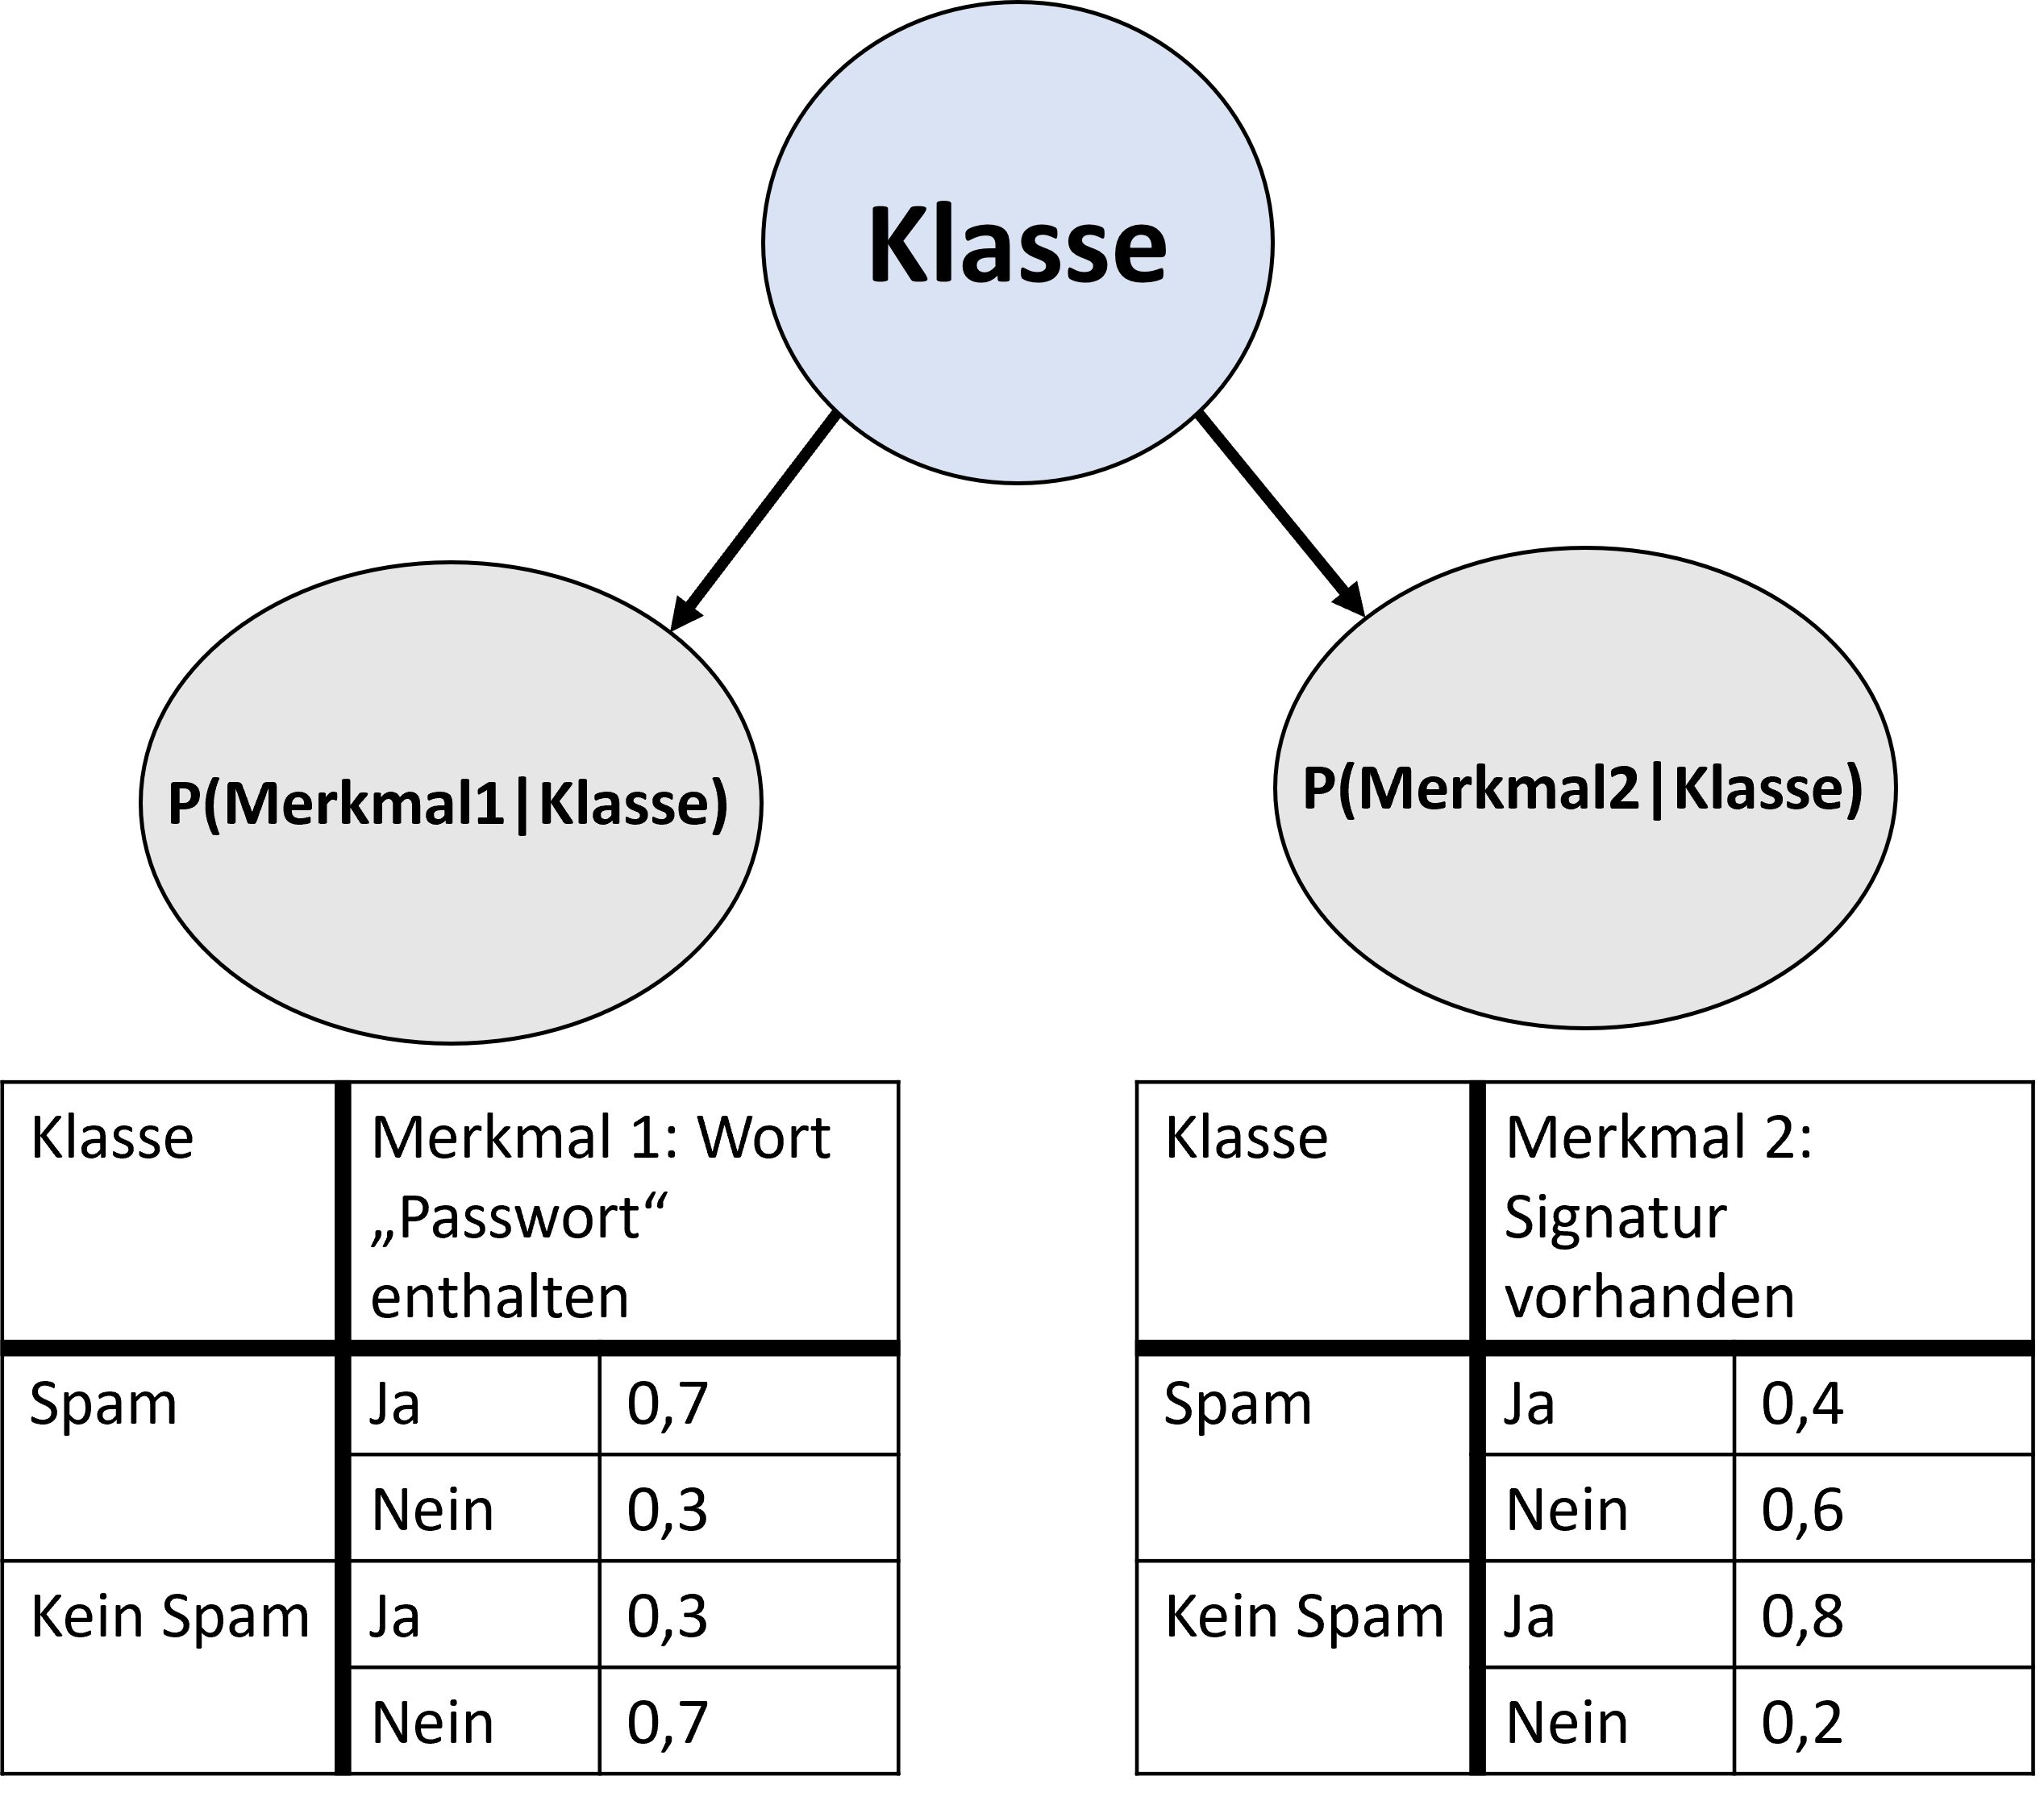
\includegraphics[scale=0.39]{pic/MA-Bilder/naivebayes.png}}
    \caption{Naive-Bayes-Klassifikator, eigene Darstellung}
    \label{Fig:naivebayes}
\end{wrapfigure}
Der Naive-Bayes-Klassifikator stellt die simpelste Ausprägung der bayesschen Netze dar \cite{Dorn.2018}. Hierbei wird für einer Entität die wahrscheinlichste Klassenzugehörigkeit ermittelt. Ein Anwendungsbeispiel, welches in Abbildung \ref{Fig:naivebayes} illustriert ist, besteht darin, festzustellen, ob es sich bei einer E-Mail um Spam oder eine legitime Nachricht handelt. Attribute der E-Mail, welche für die Zuordnung wesentlich sind, sind bestimmte Wörter oder Eigenschaften, wie das Fehlen einer Signatur. Zur Implementierung eines Naive-Bayes-Klassifikators würde ein Entwickler zunächst in vorliegenden Datenbanken mittels Durchzählen die entsprechenden
Wahrscheinlichkeiten bzgl. der jeweiligen Merkmale ermitteln. Dieses Ergebnis ist Beispielhaft in den jeweiligen Tabellen dargestellt. Danach kann unter Zuhilfenahme des bayeschen Satzes die Wahrscheinlichkeit bzgl. der Klassenzugehörigkeit ermittelt werden. Welche Merkmale von der E-Mail erfüllt werden, bestimmen die Klasse. In diesem Kontext sei erwähnt, dass bei der Zuordnung davon ausgegangen wird, dass es sich (anders als es bei den bayesschen Netzen der Fall ist) bei den Variablen um voneinander unabhängige Merkmale handelt \cite{Dorn.2018}.

Besonders bayessche Netze können es leisten, komplexe Beziehungen zu analysieren \cite{dehen2012bayes}. Das Ziel besteht darin, optimale Entscheidungen durch die Bestimmung von unbekannter Wahrscheinlichkeiten zu treffen \cite{Dorn.2018}. Hierbei wirkt sich das Fehlen von Informationen oder Erfahrungen weniger stark auf das Ergebnis aus, da dies mittels bekannten Werten bzgl. anderer Merkmale ausgeglichen werden kann. Somit können auch Unsicherheiten umgangen werden \cite{dehen2012bayes}. Jedoch ist das Konstruieren eines bayesschen Netzes unter Umständen sehr komplex \cite{wittig2002maschinelles}. Kritisch sei bzgl. des Naive-Bayes-Klassifikators angemerkt, dass dieser die Variablen unabhängig voneinander betrachtet und mit numerischen Variablen weniger gut umgehen kann \cite{Verdhan.2020}.

\subsubsection{Künstliche neuronale Netze}
Die Einsatzgebiete neuronaler Netze sind vielfältig, so können diese beispielsweise zur Klassifikation, Regression oder zur Bilderkennung eingesetzt werden \cite{ayodele, Ng.2018}. Beim Lernprozess der neuronalen Netze wird sich am biologische Gehirn orientiert. Gehirne setzen sich vereinfacht gesagt aus Neuronen zusammen, welche mit Synapsen verbunden sind, welche für einen Informationsaustausch sorgen. Analog zum Gehirn stellen Neuronen in künstlichen neuronalen Netzen ein grundlegendes Element dar, welche häufig in verschiedenen Schichten (engl. \emph{Layers}) angeordnet und verbunden sind \cite{Choo.2020}. Zu Beginn wird in diesem Unterkapitel auf Neuronen selbst eingegangen, worauf folgend die Grundlagen bzgl. der Strukturen und des Trainings neuronaler Netze vermittelt werden.

\begin{wrapfigure}{r}{0.5\textwidth}
    \centering
    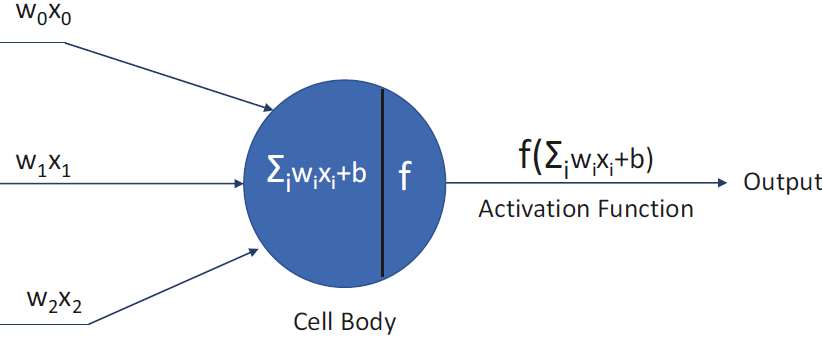
\includegraphics[scale=0.4]{pic/MA-Bilder/Neuron.PNG}
    \caption{Neuron, entnommen aus \cite{Verdhan.2020}}
    \label{Fig:neuron}
\end{wrapfigure}

\textbf{Das Neuron}

Als Grundbestandteil eines neuronalen Netzes übernimmt ein einzelnes Neuron die Aufgabe, Input eines vorangestellten Neurons zu empfangen und seinen eigenen Output zu berechnen, den es wiederum an ein weiteres Neuron weiterleitet. Wie in Abbildung \ref{Fig:neuron} illustriert, bildet ein Neuron seinen Output als Summe über alle Eingangswerte, wobei auch Gewichte der einzelnen Inputs beachtet werden und jeder Input ein anderes Gewicht haben kann \cite{Ertel.2021}. Diese Gesamtsumme der Inputs wird zusätzlich mit dem Bias-Term addiert, woraufhin das Gesamtergebnis in eine Aktiviierungsfunktion $f$ gegeben wird \cite{Ertel.2021, Verdhan.2020}. Der Einsatz verschiedenster Aktivierungsfunktionen ist im Kontext neuronaler Netze denkbar, wobei zu berücksichtigen ist, dass diese nicht-linear sein sollte. Beispiele für Aktivierungsfunktionen sind die \emph{Rectified Linear Unit}- (ReLU), die Sigmoid-Funktion oder die Softmax-Funktion, welche alle je nach Position innerhalb eines neuronalen Netzes und abhängig vom Problem, was es zu lösen gilt, unterschiedliche Vor- und Nachteile mit sich bringen \cite{Choo.2020}. Wurden innerhalb eines Neuron alle Inputdaten mithilfe der Aktivierungsfunktion bearbeitet, wird der erzeugte Output an das nächste Neuron weitergereicht und der Prozess wiederholt sich mit einem anderen Neuron \cite{Ertel.2021}.

\textbf{Strukturen neuronaler Netze}

Werden mehrere Neuronen gruppiert und verbunden, erhält man ein neuronales Netz. In einem simplen neuronalen Netz bilden die ersten und letzten Neuronen die sogenannte sichtbare Schichten, während die dazwischen liegenden Schichten als unsichtbare Sichten bezeichnet werden \cite{Choo.2020}. Bestehen Verbindungen zwischen den Schichten nur in eine Richtung, spricht man von einem \enquote{feed-forward}-Netzwerk \cite{Ertel.2021}. Ein solches ist in Abbildung \ref{Fig:neuronalesNetz} zu sehen. Bei der ersten Schicht handelt es sich um die Input-Schicht, welche die (u.U. vorverarbeiteten) Daten der Problemstellung entgegen nimmt. In dem Beispiel aus Abbildung \ref{Fig:neuronalesNetz} fließen die einzelnen Pixel des Bildes als Input in das neuronale Netz. Hierbei würde die Input-Schicht aus genau so vielen Neuronen bestehen, wie das Bild Pixel besitzt. Auf die Input-Schicht folgen verdeckte Schichten, in denen die Input-Daten nacheinander mithilfe der Neuronen transformiert werden. Die Output-Schicht als letzter Layer des neuronalen Netzes liefert das Vorhersageergebnis. Das Erscheinungsbild dieses Layers, also z.B. die Anzahl der Neuronen, ist vom zugrundeliegenden Problem und dessen Lösungsraum abhängig. In Bezug auf die verdeckten Schichten, sei angemerkt, dass mit der Anzahl der Schichten häufig auch die Präzision des Vorhersageergebnisses steigt, was jedoch zu Lasten des Rechenaufwandes geht \cite{Ng.2018}. Bei sehr vielen verdeckten Schichten spricht man häufig von DL, wobei nicht klar ist, wie viele Schichten ein künstliches neuronales Netz zu einem DL-Netz machen (vgl. Kapitel \ref{subsec_MLBegriff}). 

\begin{figure}
    \centering
    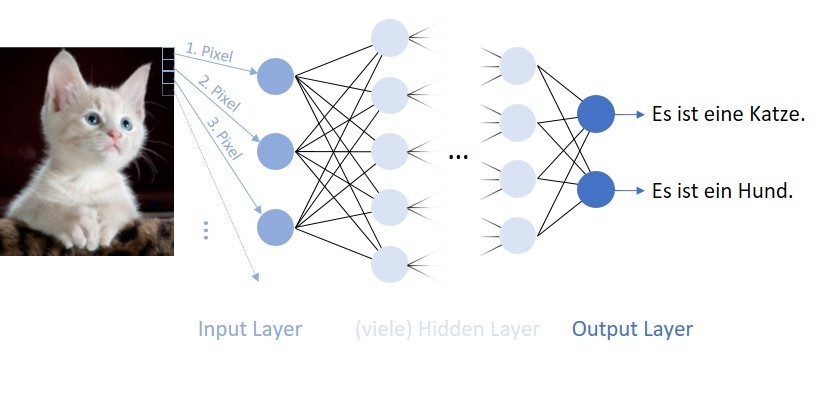
\includegraphics[scale=0.8]{pic/MA-Bilder/neuronalesNetz.jpg}
    \caption{Neuronales Netz entnommen aus \cite{MuellerKI}}
    \label{Fig:neuronalesNetz}
\end{figure}%

Neben dieser oben erläuterten Struktur neuronaler Netze existieren noch Abwandlungen, wie z.B. \emph{Convolutional Neural Network} (CNN) oder rekurrente neuronale Netzwerke \cite{Choo.2020}. Ein CNN lässt sich realisieren, indem dem neuronalen Netz nach der Input-Schicht eine oder mehrere Faltungsschichten (\emph{Conolutional Layer}) sowie \emph{Pooling}-Schichten hinzugefügt werden \cite{Ng.2018, Choo.2020}. Die Faltungsschicht hat zum Ziel lokale Muster zu finden, während das Pooling dafür verantwortlich ist, die Datenfülle zu reduzieren, da hierbei jedes Neuron nur die relevantesten Information an ihre jeweiligen Nachbarn weitergibt. CNNs werden häufig zur Bilderverarbeitung eingesetzt, da die Information, welche Pixel in einem Bild der Daten nebeneinander liegen, genutzt werden kann. Daneben existieren noch rekurrente neuronale Netzwerke als Sonderform der neuronalen Netze, welche besonders gut für die Analyse von zeitlichen Abfolge, wie z.B. Wetterdaten verwendet werden können. Hier wird nicht der gesamte Input auf einmal, sondern elementweise im Netzwerk verarbeitet. Zusätzlich verfügt jedes Neuron über einen eigenen Speicher, um Informationen über das vorherige Element nicht zu vergessen \cite{Choo.2020}.

\textbf{Training neuronaler Netze}

Beim Trainieren eines neuronalen Netzes steht die Anpassung der Gewichte und der Bias-Terme im Vordergrund. Da die Neuronen eigene Gewichte und eigenen Bias-Terme besitzen, besteht die besondere Herausforderung beim Trainieren darin, diese vielen, unterschiedlichen Parameter anzupassen. Zum Lernen wird eine Verlustfunktion (engl.: \emph{loss function}) eingesetzt, welche messen kann, inwieweit die durch das Netzwerk errechnete Antwort von der korrekten, realen Antwort abweicht \cite{Choo.2020}. Der Prozess der Anpassung der Gewichte und Bias-Vektoren selbst wird als \emph{Backpropagation} (dt.: Rückverfolgung) bezeichnet. Trifft das neuronale Netz eine falsche Vorhersage in der Output-Schicht, erfolgt eine Rückverfolgung des Fehlers und die Parameter werden insoweit angepasst, dass sich der Wert der Kostenfunktion reduziert, was wiederum eine Reduktion des inhaltlichen Fehlers zur Folge hat. Dieses Training wird meist in mehreren Runden durchlaufen \cite{Ng.2018}.

Das Potenzial der neuronalen Netze, welche das menschliche Gehirn abbilden, ist groß und bietet vielfältige Einsatzmöglichkeiten, während gleichzeitig bei der Implementation einige Herausforderungen bestehen. Analog zu den bereits betrachteten Verfahren, hängt die Funktionsweise stark von der Anzahl der vorhanden Trainingsdaten ab. Besonders, wenn das Netz komplexe Strukturen abbilden soll, und wenig Trainingsdaten vorhanden sind, neigt es zu Überanpassung \todo{Überanpassung ggf. einführen}. Weiter erfordert das Training neuronaler Netze einen hohen Rechenaufwand, der mit jedem zusätzlichen Neuron ansteigt. Ein weiterer Nachteil von neuronalen Netzen besteht darin, dass diese sich von Menschen nur schwer interpretieren lassen. Bei hundert Schichten mit mehreren Neuronen und individuellen Aktivierungsfunktionen sowie Parametern, lässt sich kaum nachvollziehen, wie ein neuronales Netzwerk zu seiner Vorhersage gelangt ist \cite{Ng.2018}. Eine Lösung für dieses Problem der Uninterpretierbarkeit bietet das erklärbare ML, das in folgenden Absätzen kurz dargestellt wird. 